\documentclass[xcolor=pdftex,dvipsnames,table,mathserif,aspectratio=169]{beamer}
\usetheme{default}
%\usetheme{Darmstadt}
%\usepackage{times}
%\usefonttheme{structurebold}

\usepackage[english]{babel}
%\usepackage[table]{xcolor}
\usepackage{pgf,pgfarrows,pgfnodes,pgfautomata,pgfheaps}
\usepackage{amsmath,amssymb,setspace,centernot}
\usepackage[latin1]{inputenc}
\usepackage[T1]{fontenc}
\usepackage{relsize}
\usepackage{pdfpages}
\usepackage[absolute,overlay]{textpos} 


\newenvironment{reference}[2]{% 
  \begin{textblock*}{\textwidth}(#1,#2) 
      \footnotesize\it\bgroup\color{red!50!black}}{\egroup\end{textblock*}} 

\DeclareMathSizes{10}{10}{6}{6} 
\AtBeginSection[]{
  \begin{frame}
  \vfill
  \centering
  \begin{beamercolorbox}[sep=8pt,center,shadow=true,rounded=true]{title}
    \usebeamerfont{title}\insertsectionhead\par%
  \end{beamercolorbox}
  \vfill
  \end{frame}
}
\begin{document}
\title{Week 3: Demand Estimation}
\author{Chris Conlon}
\institute{Grad IO}
\date{\today}

\frame{\titlepage}

\section{Heterogeneity and Endogeneity}

\begin{frame}
\frametitle{Putting it Together}
 \begin{itemize}
\item Now we want to have both \alert{price endogeneity} and \alert{flexible substitution} in the same model.
\item We are ultimately going with the random coefficients logit model, but we will start with the logit and nested logit.
 \end{itemize}
\end{frame}

\begin{frame}
\frametitle{Basic Idea from Price Endogeneity}
\begin{eqnarray*}
s_{jt} &=& \int \frac{\exp[x_{jt} \beta_i  ]}{1+\sum_k \exp[x_{kt} \beta_i ]} f(\beta_i | \theta)
\end{eqnarray*}
\begin{itemize}
\item We know prices are set with demand in mind and this can create an endogeneity problem.
\item How do we deal with it?
\item We would like to instrument in this world but what is the error term exactly?
\item An obvious choice might be $\eta_{jt} = (s_{jt}(\theta)-\tilde{s}_{jt} )$
\item Can we find things that are orthogonal to the error between observed and predicted market shares?
\item Do we have the usual IV conditions (exogeneity, relevance, monotonicity, etc.)
\end{itemize}
\end{frame}



\begin{frame}
\frametitle{Basic Idea from Price Endogeneity}
 \begin{itemize}
\item We need to add an unobservable quality term $\xi_{jt}$ to our model
\begin{eqnarray*}
u_{ijt} &=& x_{jt} \beta_i + \xi_{jt} +  \varepsilon_{ij} \\
s_{jt} &=& \int \frac{\exp[x_{jt} \beta_i + \xi_{jt} ]}{1+\sum_k \exp[x_{kt} \beta_i + \xi_{kt} ]} f(\beta_i | \theta)
\end{eqnarray*}
\item The idea is that $\xi_{jt}$ is observed to the firm when prices are set, but not to us the econometricians.
\item We call $\xi_{jt}$ a vertical component, because all consumers agree on its value.
\item This allows for products $j$ to better than some other product in a way that is not fully explained by differences in $x_j$ and $x_k$.
\item Basically there is something about a BMW that makes it better than a Peugeot in a way that is not fully captured by its mileage, weight, horsepower, etc. that leads to it having higher sales and/or higher prices.
 \end{itemize}
\end{frame}

\begin{frame}
\frametitle{Inversion: IIA Logit}
 \begin{itemize}
\item Think about the plain IIA logit for a minute:
\begin{eqnarray*}
u_{ijt} &=& x_{jt} \beta + \xi_{jt} +  \varepsilon_{ij} \\
s_{jt} &=& \frac{\exp[x_{jt} \beta + \xi_{jt} ]}{1+\sum_k \exp[x_{kt} \beta + \xi_{kt} ]} 
\end{eqnarray*}
\item Take logs
\begin{eqnarray*}
\ln s_{0t} &=& -\log \left(1+\sum_k \exp[x_{kt} \beta + \xi_{kt}] \right) \\
\ln s_{jt} &=& [x_{jt} \beta + \xi_{jt} ] - \log \left(1+\sum_k \exp[x_{kt} \beta + \xi_{kt}] \right)\\
\ln s_{jt}- \ln s_{0t} &=& x_{jt} \beta -\alpha p_{jt} +  \xi_{jt}
\end{eqnarray*}
 \end{itemize}
\end{frame}

\begin{frame}
\frametitle{Inversion: IIA Logit}
\begin{eqnarray*}
\underbrace{\ln s_{jt}- \ln s_{0t}}_{data!}&=& \underbrace{x_{jt} \beta -\alpha p_{jt} +  \xi_{jt}}_{\delta_{jt}}
\end{eqnarray*}
 \begin{itemize}
\item The LHS is data! The RHS is now a linear IV problem!
\item $\alpha$ the price coefficient is the endogenous parameter.
\item We know how to solve this. We need instruments that shift $p_{jt}$ but are orthogonal to $\xi_{jt}$.
\item Economic theory tells us how: cost shifters, markup shifters.
\item Markups in IIA logit are pretty boring since they only depend on your shares and $\alpha$.
\item If number of products varies across markets, that works. Otherwise you want cost shifters in cross section or time series.
 \end{itemize}
\end{frame}


\begin{frame}
\frametitle{Was that magic?}
\begin{itemize}
\item No. It was just a nonlinear change of variables from $\eta_{jt} \rightarrow \xi_{jt}$.
\item Our moment condition is just that $E[\xi_{jt} | x_{jt}, z_{jt}]=0$.
\item We moved from the space of shares and MLE for the logit to the space of utilities and an IV model.
\item We are losing some efficiency -- but now we are able to estimate under weaker conditions.
 \end{itemize}
\end{frame}

\begin{frame}
\frametitle{Caveats}
\begin{itemize}
\item We do need a technical condition. This only works if the market size $N \rightarrow \infty$.
\item That is our data/shares we must believe we are observing without any sampling error.
\item This is not necessary for the multinomial MLE where shares have some natural sampling variation.
\item In our IV/GMM approach we cannot have this sampling error. (Why?).
 \end{itemize}
\end{frame}


\begin{frame}
This takes a bit more algebra but not much
\frametitle{Inversion: Nested Logit (Berry 1994 / Cardell 1991)}
\begin{eqnarray*}
\underbrace{\ln s_{jt}- \ln s_{0t}}_{data!}&=& x_{jt} \beta -\alpha p_{jt} - \sigma \underbrace{\log(s_{j|gt})}_{data!}+  \xi_{jt}
\end{eqnarray*}
 \begin{itemize}
\item Same as logit plus an extra term $\log(s_{j|g})$ the \alert{within group share}.
\item We now have a second endogenous parameter.
\item If you don't see it -- realize we are regressing $Y$ on a function of $Y$. This should always make you nervous.
\item If you forget to instrument for $\sigma$ you will get $\sigma \rightarrow 1$ because of \alert{attenuation bias}.
\item A good instrument for $\sigma$ is the number of products within the nest. Why?
 \end{itemize}
\end{frame}

\begin{frame}
\frametitle{Inversion: BLP}
We can't solve for $\delta_{jt}$ directly this time. We often exploit a trick when $\beta_i,\nu_i$ is normally distributed:
\begin{eqnarray*}
s_{jt} &=& \int \frac{\exp[\delta_{jt} + x_{jt} \cdot\Sigma \cdot \nu_i ]}{1+\sum_k \exp[\delta_{kt} +  x_{kt} \cdot\Sigma \cdot \nu_i  ]} f(\nu_i | \theta)
\end{eqnarray*}
 \begin{itemize}
 \item This is a $J \times J$ system of equations for each $t$.
 \item It is diagonally dominant.
 \item There is a unique vector $\xi_t$ that solves it for each market $t$.
 \item If you can work out $\frac{\partial s_{jt}}{\partial \delta_{kt}}$ (easy) you can solve this using Newton's Method.
 \end{itemize}
\end{frame}

\begin{frame}
\frametitle{Contraction: BLP}
BLP actually propose an easy solution to find $\delta_t$. Fix $\theta$ and solve for $\delta$. Think about doing this one market at a time:
\begin{eqnarray*}
\delta^{(k)}(\theta) = \delta^{(k-1)}(\theta) + \log(\tilde{s}_{j}) - \log(s_{j}(\delta_t^{(k-1)}, \theta)
\end{eqnarray*}
 \begin{itemize}
 \item They prove (not easy) that this is a \alert{contraction mapping}.
 \item If you keep iterating this equation enough $|\delta^{(k)}(\theta) - \delta^{(k-1)}(\theta)| < \epsilon_{tol}$ you can recover the $\delta$'s so that the observed shares and the predicted shares are identical.
 \item Practical tip: $\epsilon_{tol}$ needs to be as small as possible. ($\approx 10^{-13}$).
 \item Practical tip: Contraction isn't as easy as it looks:  $ \log(s_{j}(\delta_t^{(k-1)}, \theta)$ requires computing the numerical integral each time (either via quadrature or monte carlo).
  \end{itemize}
 \end{frame}
 
 
 \begin{frame}
\frametitle{BLP Pseudocode}
From the outside, in:
\begin{itemize}
\item Outer loop: search over nonlinear parameters $\theta$ to minimize GMM objective:
 \begin{eqnarray*}
 \widehat{\theta_{BLP}} = \arg \max_{\theta} (Z' \hat{\xi}(\theta)) W  (Z' \hat{\xi}(\theta))'
 \end{eqnarray*}
 \item Inner Loop:
 \begin{itemize}
\item Fix $\theta$.
\item Solve for $\delta$ so that $s_{jt}(\delta,\theta) = \tilde{s}_{jt}$.
\begin{itemize}
\item Computing $s_{jt}(\delta,\theta)$ requires numerical integration (quadrature or monte carlo).
\end{itemize}
 \item We can do IV-GMM to recover $\hat{\alpha}(\theta),\hat{\beta}(\theta),\hat{\xi}(\theta)$.
  \begin{eqnarray*}
\delta_{jt}= x_{jt} \beta -\alpha p_{jt}+  \xi_{jt}
 \end{eqnarray*}
  \item Use $\hat{\xi}(\theta)$ to construct moment conditions.
 \end{itemize}
 \item When we have found $\hat{\theta}_{BLP}$ we can use this to update $W \rightarrow W(\hat{\theta}_{BLP})$ and do 2-stage GMM.
 \end{itemize}
\end{frame}




 \begin{frame}
\frametitle{BLP Estimation}
\begin{itemize}
 \item Now that you have done change of variables to get:
 \begin{eqnarray*}
\delta_{jt}= x_{jt} \beta -\alpha p_{jt}+  \xi_{jt}
 \end{eqnarray*}
 \item We can do IV-GMM to recover $\hat{\alpha}(\theta),\hat{\beta}(\theta),\hat{\xi}(\theta)$.
 \item Outer Loop update guess $\theta$, solve for $\delta$ and repeat.
 \begin{eqnarray*}
 \widehat{\theta_{BLP}} = \arg \max_{\theta} (Z' \hat{\xi}(\theta)) W  (Z' \hat{\xi}(\theta))'
 \end{eqnarray*}
 \item When we have found $\hat{\theta}_{BLP}$ we can use this to update $W \rightarrow W(\hat{\theta}_{BLP})$ and do 2-stage GMM.
 \end{itemize}
\end{frame}



 \begin{frame}
\frametitle{BLP Alternatives}
\begin{itemize}
 \item BLP give us both a statistical \alert{estimator} and an \alert{algorithm} to obtain estimates.
\item Plenty of other algorithms exist
\begin{itemize}
\item We could solve for $\delta$ using the contraction mapping, using \texttt{fsolve} / Newton's Method / Guess and Check (not a good idea!).
\item We could try and consider a non-nested estimator for the BLP problem instead of solving for $\delta(\theta),\xi(\theta)$ we could let $\delta,\xi,\alpha,\beta$ be free parameters.
 \end{itemize}
\item We could think about different statistical estimators such as $K$-step GMM, Continuously Updating GMM, etc.
 \end{itemize}
\end{frame}
 \begin{frame}
 
\begin{eqnarray}
\frametitle{Dube Fox Su (2012)}
\label{blpnfxp}
\nonumber \arg \min_{\theta_2} && \psi' \Omega^{-1} \psi \quad \mbox{ s.t. } \\
\nonumber \psi &=& \xi(\theta_2)' Z\\
\xi_{jt}(\theta) &=& \delta_j(\theta_2) - x_{jt} \beta - \alpha p_{jt} \\
\nonumber \log(S_{jt})  &=& \log(s_{jt}(\delta,\theta_2))
\end{eqnarray}

\begin{eqnarray}
\label{blpmpec}
\nonumber \arg \min_{\theta_2,\alpha,\beta, \xi,\psi} && \psi' \Omega^{-1}  \psi \quad \mbox{ s.t. } \\
 \psi &=& \xi' Z\\
\nonumber \log(S_{jt})  &=& \log(s_{jt}(\xi,\theta_2, \alpha, \beta))
\end{eqnarray}
\end{frame}

\begin{frame}
\frametitle{Comparing Approaches}
\begin{itemize}
\item The original BLP paper and the DFS paper define different \alert{algorithms} to produce the same statistical \alert{estimator}.
\begin{itemize}
\item The BLP algorithm is a \alert{nested fixed point} (NFP) algorithm. 
\item The DFS algorithm is a \alert{mathematical program with equilibrium constraints} (MPEC).
\item The unknown parameters satisfy the same set of first-order conditions. (Not only asymptotically, but in finite sample).
\item $\hat{\theta}_{NFP} \approx \hat{\theta}_{MPEC}$ but for numerical differences in the optimization routine.
\end{itemize}
\item Our choice of algorithm should mostly be about computational convenience.
\end{itemize}
\end{frame}

\begin{frame}
\frametitle{BLP: NFP Advantages/Disadvantages}
\begin{itemize}
\item Advantages
\begin{itemize}
\item Concentrate out all of the linear in utility parameters $(\xi,\delta,\beta)$ so that we only search over $\Sigma$. When $\dim(\Sigma)=K$ is small (few dimensions of unobserved heterogeneity) this is a big advantage. For $K \leq 3$ this is my preferred approach.
\item When $T$ (number of markets/periods) is large then you can exploit solving in parallel for $\delta$ market by market.
\end{itemize}
\item Disadvantages
\begin{itemize}
\item Small numerical errors in contraction can be amplified in the outer loop, $\rightarrow$ tolerance needs to be very tight.
\item Errors in numerical integration can also be amplified in the outer loop $\rightarrow$ must use a large number of draws/nodes.
\item Hardest part is working out the Jacobian via IFT.
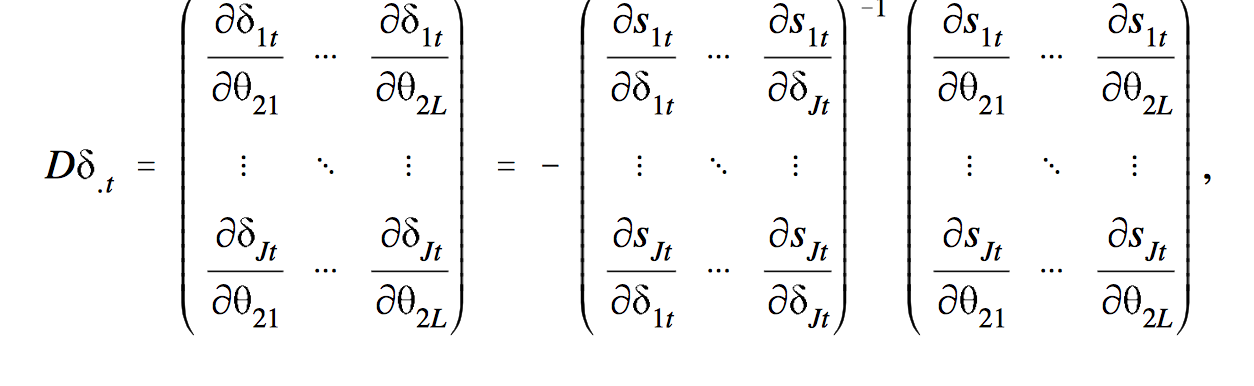
\includegraphics[width=2.8in]{resources/implicit_function.png}\\
\end{itemize}
\end{itemize}
\end{frame}

\begin{frame}
\frametitle{BLP: MPEC Advantages/Disadvantages}
\begin{itemize}
\item Advantages
\begin{itemize}
\item Problem scales better in $\dim(\Sigma)$.
\item Because all constraints hold at the optimum only: less impact of numerical error in tolerance or integration.
\item Derivatives are less complicated than $\frac{\partial \delta}{\partial \theta}$ (no IFT).
\end{itemize}
\item Disadvantages
\begin{itemize}
\item We are no longer concentrating out parameters, so there are a lot more of them! Storing the (Hessian) matrix of second derivatives can be difficult on memory.
\item We have to find the derivatives of the shares with respect to all of the parameters $\beta,\xi,\theta$. (The other derivatives are pretty easy).
\item Parallelizing the derivatives is trickier than NFP case.
\end{itemize}
\end{itemize}
\end{frame}


\begin{frame}
\frametitle{BLP Extensions: Demographics}
\begin{itemize}
\item It is helpful to allow for interactions with consumer demographics (such as income).
\begin{eqnarray*}
\alpha_{it} = \overline{\alpha} + \sigma_p \nu_i + \pi_p y_{it}
\end{eqnarray*}
\item A few ways to do this:
\begin{itemize}
\item You could just use cross sectional variation in $s_{jt}$ and $\overline{y}_t$ (mean or median income).
\item Better: Draw $y_{it}$ from a geographic specific income distribution. Draw $\nu_i$ from a general distribution of unobserved heterogeneity.
\end{itemize}
\item Ex: Nevo (2000) Cereal demand sampled individual level $D_i$ from geographic specific CPS data
\item Joint distribution of income, income-squared, age, child at home.
\begin{eqnarray*}
\beta_i = \overline{\beta} + \Pi D_i + \sigma \nu_i
\end{eqnarray*}
\end{itemize}
\end{frame}

\begin{frame}
\frametitle{BLP Extensions: Panel Data}
\begin{itemize}
\item with enough observations on the same product it is possible to include fixed effects
\begin{eqnarray*}
\delta_{jt}(\Sigma) = x_{jt} \beta - \alpha p_{jt} + \underbrace{\xi_{jt}}_{\xi_{j} + \xi_t + \Delta \xi_{jt}}
\end{eqnarray*}
\item What does $\xi_{j}$ mean in this context?
\item What would $\xi_t$ mean in this context?
\item $\Delta \xi_{jt}$ is now the structural error term, this changes our identification strategy a little.
\end{itemize}
\end{frame}

\begin{frame}
\frametitle{Extensions: Micro Data (Petrin 2002), (microBLP 2004)}
Suppose we had additional data on behavior of individuals (in addition to aggregate market).
\begin{itemize}
\item Examples:
\begin{itemize}
\item For some customers have answer to ``Which car would you have purchased if the car you bought was not available?''
\item Demographic data on purchasers of a single brand.
\item Full individual demographic and choice data.
\end{itemize}
\end{itemize}
\end{frame}

\begin{frame} \frametitle{Extensions: Micro Data (Petrin 2002), (microBLP 2004)}
\begin{itemize}
\item Previously we had moment conditions from orthogonality of structural error $(\xi)$ and $(X,Z)$ in order to form our GMM objective.
\begin{eqnarray*}
E[\xi_{jt} | x_{jt}, z_{jt}]=0 \rightarrow E[\xi'  [Z \, X]]=0
\end{eqnarray*}
\item We can incorporate additional information using ``micro-moments'' or additional moment conditions to match the micro data.
\begin{itemize}
\item $Pr(\mbox{ i buys j } | y_i \in [0,\$20K])= c_1$
\item $Cov(d_i, s_{ijt}) = c_2$
\item Construct an additional error term $\zeta_1,\zeta_2$ and interact that with instruments to form additional moment conditions.
\item Econometrics get tricky when we have a different number of observations for $E[\zeta' [X Z]]=0$ and $E[\xi' [X Z]]=0$.
\end{itemize}
\end{itemize}
\end{frame}

\begin{frame}
\frametitle{Alternative: Vertical Model (Bresnahan 1987)}
\begin{itemize}
\item Imagine everyone agreed on the quality of the products offered for sale.
\item The only thing people disagree on is willingness to pay for quality
\begin{eqnarray*}
U_{ij} = \overline{u} + \delta_j - \alpha_i p_j
\end{eqnarray*}
\item How do we estimate?
\begin{itemize}
\item Sort goods from $p_1 < p_2  < p_3 \ldots < p_J$.\\
 It must be that $\delta_1 < \delta_2 < \ldots < \delta_J$. Why?
 \item Normalize o.g. to $0$ so that $ 0 > \delta_1 -\alpha_i p_1$ or $\alpha_i > \delta_1 / p_1$.
 \item $s_0 = F(\infty) - F(\frac{\delta_1}{p_1})  = 1 - F(\frac{\delta_1}{p_1}) $ where $F(\cdot)$ is CDF of $\alpha_i$.
 \item In general choose $j$ IFF:
 \begin{eqnarray*}
 \frac{\delta_{j+1} - \delta_j}{p_{j+1} -p_j} < \alpha_i < \frac{\delta_j  - \delta_{j-1}}{p_j - p_{j-1}}\\
 s_j = F\left(\frac{\delta_{j+1} - \delta_j}{p_{j+1} -p_j} \right) - F\left(\frac{\delta_j  - \delta_{j-1}}{p_j - p_{j-1}} \right)
 \end{eqnarray*}
\end{itemize}
\end{itemize}
\end{frame}

\begin{frame}
\frametitle{Alternative: Vertical Model (Bresnahan 1987)}
Estimation
\begin{itemize}
\item Choose parameters $\theta$ of $F(\cdot)$ in order to best match $s_j$.
\begin{itemize}
\item Can do MLE $\arg \max_{\theta} \sum_j \tilde{s}_j \log s_{j}(\theta)$.
\item Can do least squares $\sum_j (\tilde{s}_j - s_{j}(\theta) )^2$.
\item Can do IV/GMM if I have an instrument for price.  $\delta_j = x_j \beta + \xi_j$.
\item Extremely easy when $F\sim \exp(\lambda)$.
\end{itemize}
\item What about elasticities?
\begin{itemize}
\item When I change the price of $j$ it can only affect $(s_{j-1},s_j, s_{j+1})$.
\item We have set all of the other cross-price elasticities to be zero.
\item If a luxury car and a truck have similar prices, this can create strange substitution patterns.
\end{itemize}
\end{itemize}
\end{frame}

\begin{frame} \frametitle{Pure Characteristics Model: Berry Pakes (2001/2007)}
\footnotesize
\begin{eqnarray*}
u_{ij} = \delta_j + \sum_k \nu_{ik} x_{jk} + \xi_{j} + \underbrace{\sigma_i \epsilon_{ij}}_{\rightarrow 0}
\end{eqnarray*}
\begin{itemize}
\item Can think of this like random coefficients model where we take the variance of $\epsilon$ to zero.
\item Can think of this a vertical model, with vertical tastes over several characteristics.
\begin{itemize}
\item PCs: everyone prefers more Mhz, more RAM, and more storage but differ in WTP.
\item Possible that there is no PC specific $\epsilon$.
\end{itemize}
\item Advantages
\begin{itemize}
\item Logit error means there is always some substitution to all other goods. 
\item Reality may be you only compete with a small number of competitors.
\item Allows for \alert{crowding} in the product space.
\end{itemize}
\item Disadvantage: no closed form for $s_j$, so estimation is extremely difficult.
\item Minjae Song (Homotopy) and Che-Lin Su (MPCC) have made progress using two different approaches.
\end{itemize}
\end{frame}

\section{Adding Supply}
\begin{frame}{Supply}
\begin{itemize}
\item Economic theory gives us some additional powerful restrictions.
\item We may want to impose $MR = MC$.
\item Alternatively, we can ask -- what is a good instrument for demand? \alert{something from another equation} (ie: supply).
\end{itemize}
\end{frame}

\begin{frame}{Bertrand Nash Pricing}
Consider the problem of firm $f$ which sets prices $p_j$ for products in the set $\mathcal{J}_f$:
\begin{eqnarray*}
\arg \max_{p \in \mathcal{J}_f} \pi_f (\mathbf{p}) &=& \sum_{j \in \mathcal{J}_f} (p_j - c_j) \cdot q_j(\mathbf{p}) \\
\rightarrow 0&=& q_j(\mathbf{p}) + \sum_{k \in \mathcal{J}_f} (p_k - c_k) \frac{\partial q_{k}}{\partial p_j}(\mathbf{p})
\end{eqnarray*}
We can re-write the FOC in matrix form:
\begin{eqnarray*}
q(\mathbf{p}) = \Omega(\mathbf{p})\cdot(\mathbf{p}-\mathbf{mc})
\end{eqnarray*}
\end{frame}

\begin{frame}{Bertrand Nash Pricing (cont)}
It is helpful to define two $J_t \times J_t$ matrices. The first is an \textit{ownership matrix}:
\begin{eqnarray*}
O_{(j,k)} = \left\{\begin{array}{lr}
          1 & \text{for }  (j,k) \in \mathcal{J}_f\\
       	  0 & \text{for } (j,k) \notin \mathcal{J}_f
        \end{array} \right\}
\end{eqnarray*}
And the second is the matrix of demand derivatives $\tilde{\Omega}(\mathbf{p})$ with entries $\tilde{\Omega}_{(j,k)}(\mathbf{p})=\frac{\partial q_{j}}{\partial p_k}(\mathbf{p})$. We are mainly interested in the Hadamard (element-wise) product of the two matrices $\Omega = O\bigodot\tilde{\Omega}$.
\begin{eqnarray*}
\Omega_{(j,k)}(\mathbf{p},\theta) = \left\{\begin{array}{lr}
         - \frac{\partial q_{j}}{\partial p_k}(\mathbf{p},\theta) & \text{for }  (j,k) \in \mathcal{J}_f\\
       	  \quad 0 & \text{for } (j,k) \notin \mathcal{J}_f
        \end{array} \right\}
\end{eqnarray*}
\end{frame}


\begin{frame}{Recovering Marginal Costs }
Recover implied markups/ marginal costs, and assume a functional form for $mc_{jt}(x_{jt},w_{jt})$.
\begin{eqnarray*}
\widehat{\mathbf{mc}}(\theta)&=& \mathbf{p}- \Omega(\mathbf{p},\theta)^{-1} q(\mathbf{p},\theta)\\
f(mc_{jt}) &=& x_{jt} \gamma_1 + w_{jt} \gamma_2 + \omega_{jt}
\end{eqnarray*}
Which we can solve for $\omega_{jt}$:
\begin{eqnarray*}
\omega_{jt} &=&  f(\mathbf{p}- \Omega(\mathbf{p},\theta)^{-1} q(\mathbf{p},\theta)) - x_{jt} \gamma_1 - w_{jt} \gamma_2
\end{eqnarray*}
\begin{itemize}
\item $f(\cdot)$ is usually $\log(\cdot)$ or identity.
\item I can use this to form additional moments: $E[\omega_{jt}' Z_{jt}^{s}]=0$.
\item I can just stack these up with the demand moments $E[\xi_{jt}' Z_{jt}^d]=0$.
\item Now I have $\dim(Z^d) + \dim(Z^s)$ moments altogether.
\item This step is optional but can aid in identification (if you believe it).
\end{itemize}

\end{frame}

\begin{frame}{Supply Side as Instruments }
\begin{itemize}
\item Instruments for demand depend on \alert{exclusion restrictions}
\item Where do instruments come from? Something omitted that appears in another equation.
\end{itemize}
\begin{eqnarray*}
p_{jt}  &=& c_{jt}(w_{jt},x_{jt}) +  \frac{s_{jt}(\mathbf{p_t})}{\left|\frac{\partial s_{jt}(\mathbf{p_t})}{\partial p_{jt}}\right|}  +\sum_{k \in \mathcal{J}_f} (p_k - c_k) \frac{\frac{ \partial s_{kt}}{\partial p_{jt}}(\mathbf{p_t})}{\left|\frac{\partial s_{jt}(\mathbf{p_t})}{\partial p_{jt}}\right|}  
\end{eqnarray*}
\begin{enumerate}
\item Exogenous regressors $x_{jt}$.
\item Cost shifters: $w_{jt}$ (hard to find in practice), Hausman instruments.
\item Markup shifters:  $ \frac{s_{jt}(\mathbf{p_t})}{\frac{\partial s_{jt}(\mathbf{p_t})}{\partial p_{jt}}}$ \\(function of $(p_j,x_j,\xi_j, p_{-j},x_{-j},\xi_{-j})$).
\end{enumerate}
\end{frame}


\section{Instruments and Identification}

\begin{frame}{Instruments}
\begin{itemize}
\item Recall the nested logit, where there are two separate endogeneity problems
\begin{itemize}
\item \alert{Price}: this is the familiar one!
\item \alert{Nonlinear characteristics} $\sigma$ this is the other one.
\end{itemize}
\item We are doing nonlinear GMM: Start with $E[\xi_{jt} | x_{jt}, z_{jt}]=0$ use $E[\xi' [Z X]]=0$.
\begin{itemize}
\item In practice this means that for valid instruments $(x,z)$ any function $f(x,z)$ is also a valid instrument $E[ \xi_{jt} f(x_{jt},z_{jt})]=0$.
\item We can use $x, x^2, x^3,\ldots$ or interactions $x \cdot z, x^2 \cdot z^2, \ldots$.
\item What is a reasonable choice of $f(\cdot)$?
\item Where does $z$ come from?
\end{itemize}
\end{itemize}
\end{frame}

\begin{frame}{Identifcation}
\begin{itemize}
\item Once we have $\delta_{jt}(\theta)$ identification of linear parameters is pretty straightforward
\begin{eqnarray*}
\delta_{jt}(\theta) = x_{jt} \beta - \alpha p_{jt} + \xi_j + \xi_t + \Delta \xi_{jt}
\end{eqnarray*}
\item This is either basic linear IV or panel linear IV.
\item How are $\sigma$ taste parameters identified?
\begin{itemize}
\item Consider increasing the price of $j$ and measuring substitution to other products $k,k'$ etc.
\item If sales of $k$ increase with $p_j$ and $(x_j^{(1)},x_k^{(1)})$ are similar then we increase the $\sigma$ that corresponds to $x^{(1)}$.
\item Price is the most obvious to vary, but sometimes this works for other characteristics (like distance).
\item Alternative: vary the set of products available to consumers by adding or removing an option.
\end{itemize}
\end{itemize}
\end{frame}



\begin{frame} \frametitle{Extensions: Supply Moments}
\begin{itemize}
\item We can also impose the Bertrand FOC as a set of additional moments.
\item First parametrize marginal cost
\begin{eqnarray*}
\ln mc_{jt} = \gamma_1 x_{jt} + \gamma_2 w_{jt} + \omega_{jt}
\end{eqnarray*}
\item helpful to constrain MC to be positive always.
\item Note that for any vector of prices $p$ and demand parameters $\theta$ we can recover a unique vector of marginal costs (by solving the system of linear equations).
\item Imposing the supply side only helps if we have information about the marginal costs / production function that we would like to impose
\item Imposing these restrictions is helpful in constraining markups (so that implied MC are always positive, etc.).
\item Misspecified functional forms for costs can cause problems!
\end{itemize}
\end{frame}


\begin{frame}{Instruments}
\begin{itemize}
\item Common choices are average characteristics of other products in the same market $h(x_{-j,t})$. \alert{BLP instruments}
\begin{itemize}
\item Same firm $z_{1jt} = \overline{x}_{-j_f,t} = \frac{1}{\left\vert{F_j}\right\vert}  \sum_{k \in \mathcal{F}_j} x_{kt} - \frac{1}{\left\vert{F_j}\right\vert} x_{jt}$.
\item Other firms $z_{2jt}=\overline{x}_{\cdot t} - \overline{x}_{-j_f,t} - \frac{1}{J} x_{jt}$.
\item Plus regressors $(1, x_{jt})$.
\item Plus higher order interactions 
\end{itemize}
\item Technically linearly independent for large (finite) $J$, but becoming highly correlated.
\begin{itemize}
\item Can still exploit variation in number of products per market or number of products per firm.
\end{itemize}
\item Correlated moments $\rightarrow$ ``many instruments''.
\begin{itemize}
\item May be inclined to ``fix'' correlation in instrument matrix directly.
\end{itemize}
\end{itemize}
\end{frame}

\begin{frame}{Armstrong (2016): Weak Instruments?}
Consider the limit as $J \rightarrow \infty$
\begin{eqnarray*}
\frac{s_{jt}(\mathbf{p_t})}{\left|\frac{\partial s_{jt}(\mathbf{p_t})}{\partial p_{jt}}\right|} = \frac{1}{\alpha} \frac{1}{1-s_{jt}} \rightarrow \frac{1}{\alpha}
\end{eqnarray*}
\begin{itemize}
\item Hard to use markup shifting instruments to instrument for a constant.
\item How close to the constant do we get in practice?
\item Average of $x_{-j}$ seems like an especially poor choice. Why?
\item Shows there may still be some power in: products per market, products per firm.
\item Convergence to constant extends to mixed logits (see Gabaix and Laibson 2004).
\item Evidence that you really need cost shifters.
\end{itemize}
\end{frame}

\begin{frame}{Optimal Instruments}
How to construct optimal instruments in form of Chamberlain (1987)
\begin{eqnarray*}
E\left[\frac{\partial \xi_{jt}}{\partial \theta} | X_t, w_{jt} \right] = \left[\beta, E\left[\frac{\partial \xi_{jt}}{\partial \alpha} | X_t, w_{jt} \right] , E[\frac{\partial \xi_{jt}}{\partial \sigma} | X_t, w_{jt} ] \right]
\end{eqnarray*}
Some challenges:
\begin{enumerate}
\item $p_{jt}$ depends on $X_{t}, w_{t}, \xi_{t}$ in a highly nonlinear way (no explicit solution!).
\item $E[\frac{\partial \xi_{jt}}{\partial \sigma} | X_t, w_{t} ] =E[[\frac{\partial \mathbf{s_t}}{\partial \mathbf{\delta_t}}]^{-1} [\frac{\partial \mathbf{s_t}}{\partial \mathbf{\sigma}}] | X_t, w_{t} ]$  (not conditioned on endogenous $p$!)
\end{enumerate}
``Feasible'' Recipe:
\begin{enumerate}
\item Fix $\hat{\theta}=(\hat{\alpha},\hat{\beta},\hat{\sigma})$ and draw $\xi_t$ from empirical density
\item Solve fixed point equation for $\hat{p_{jt}}$
\item Compute necessary Jacobian
\item Average over all values of $\xi_t$. (Lazy approach: use only $\xi =0$).
\end{enumerate}
\end{frame}

\begin{frame}{Optimal Instruments}
\begin{itemize}
\item Since any $f(x,z)$ satisfies our orthogonality condition, we can try to choose $f(x,z)$ as a \alert{basis} to approximate optimal instruments.
\item This is challenging in practice -- and in fact suffers from a curse of dimensionality.
\item This is frequently given as a rationale behind higher order $x$'s.
\item When the dimension of $x$ is low -- this may still be feasible. ($K \leq 3)$.
\end{itemize}
\end{frame}

\begin{frame}{Optimal Instruments: Reynaert Verboven (2014)}
\begin{itemize}
\footnotesize
\item Optimal instruments are easier to work out if $p = mc$.
\begin{eqnarray*}
c = p  + \underbrace{\Delta^{-1} s}_{\rightarrow 0}  = X \gamma_1 + W \gamma_2 + \omega
\end{eqnarray*}
\item Linear cost function means linear reduced-form price function.
\begin{eqnarray*}
E\left[ \frac{\partial \xi_{jt} }{\partial \alpha} | z_t \right] &=& E[p_{jt} | z_t] = x_{jt} \gamma_1 + w_{jt} \gamma_2\\
E\left[ \frac{\partial \omega_{jt} }{\partial \alpha} | z_t \right] &=& 0 , \quad E\left[ \frac{\partial \omega_{jt} }{\partial \sigma} | z_t \right] = 0\\
E\left[ \frac{\partial \xi_{jt} }{\partial \sigma} | z_t \right] &=&E\left[ \frac{\partial \delta_{jt} }{\partial \sigma} | z_t \right]\\
\end{eqnarray*}
\item If we are worried about endogenous oligopoly markups is this a reasonable idea?
\end{itemize}
\end{frame}

\begin{frame}{Optimal Instruments: Reynaert Verboven (2014)}
\begin{center}
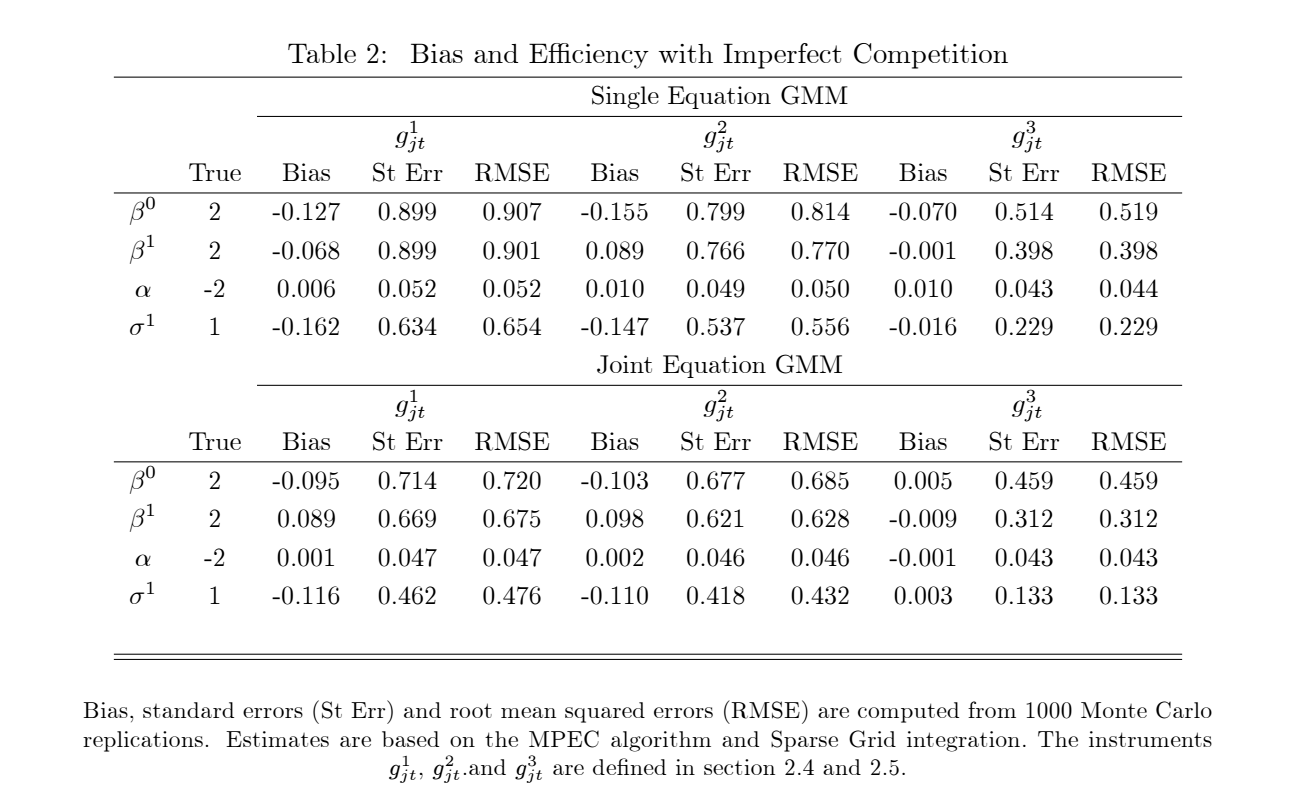
\includegraphics[width=4in]{resources/verboven.png}
\end{center}
\end{frame}


\begin{frame}{Differentiation Instruments: Gandhi Houde (2016)}
\begin{itemize}
\item Also need instruments for the $\Sigma$ or $\sigma$ random coefficient parameters.
\item Instead of average of other characteristics $h(x) = \frac{1}{J-1} \sum_{k \neq j} x_k$, can transform as distance to $x_j$.
\begin{eqnarray*}
d_{jt} ^k=  x_k - x_j  \\
\end{eqnarray*}
\item And use this transformed to construct two kinds of IV (Squared distance, and count of local competitors)
\begin{eqnarray*}
DIV_1 =& \sum_{j \in F}  d_{jt}^2,  \quad &\sum_{j \notin F}  d_{jt}^2 \\
DIV_2 =& \sum_{j \in F}  I[d_{jt} < c]   \quad &\sum_{j \notin F}   I[d_{jt} < c]
\end{eqnarray*}
\item They choose $c$ to correspond to one standard deviation of $x$ across markets.
\end{itemize}
\end{frame}


\begin{frame}{Differentiation Instruments: Gandhi Houde (2016)}
\begin{center}
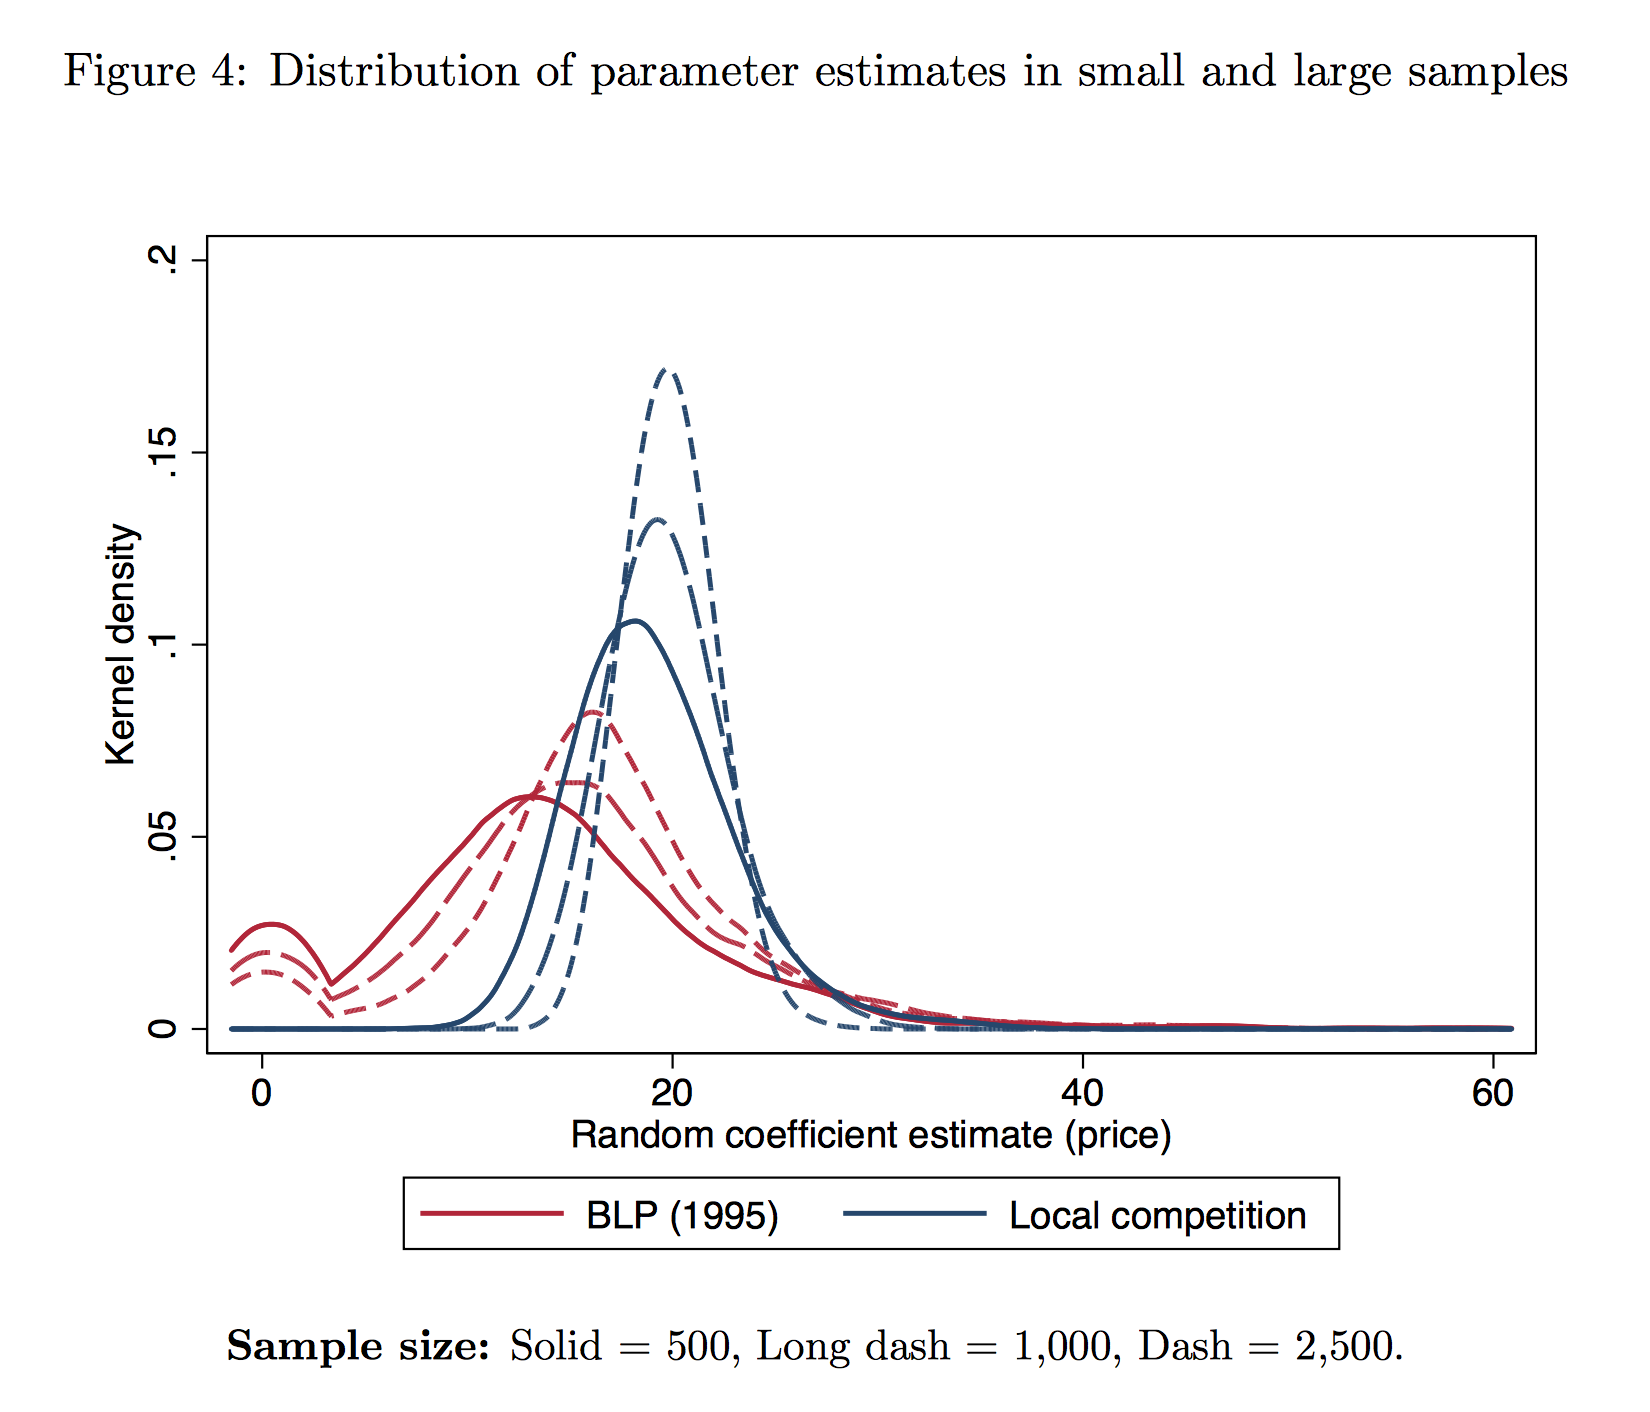
\includegraphics[width=4in]{resources/d_iv1.png}
\end{center}
\end{frame}


\begin{frame}{Differentiation Instruments: Gandhi Houde (2016)}
\begin{center}
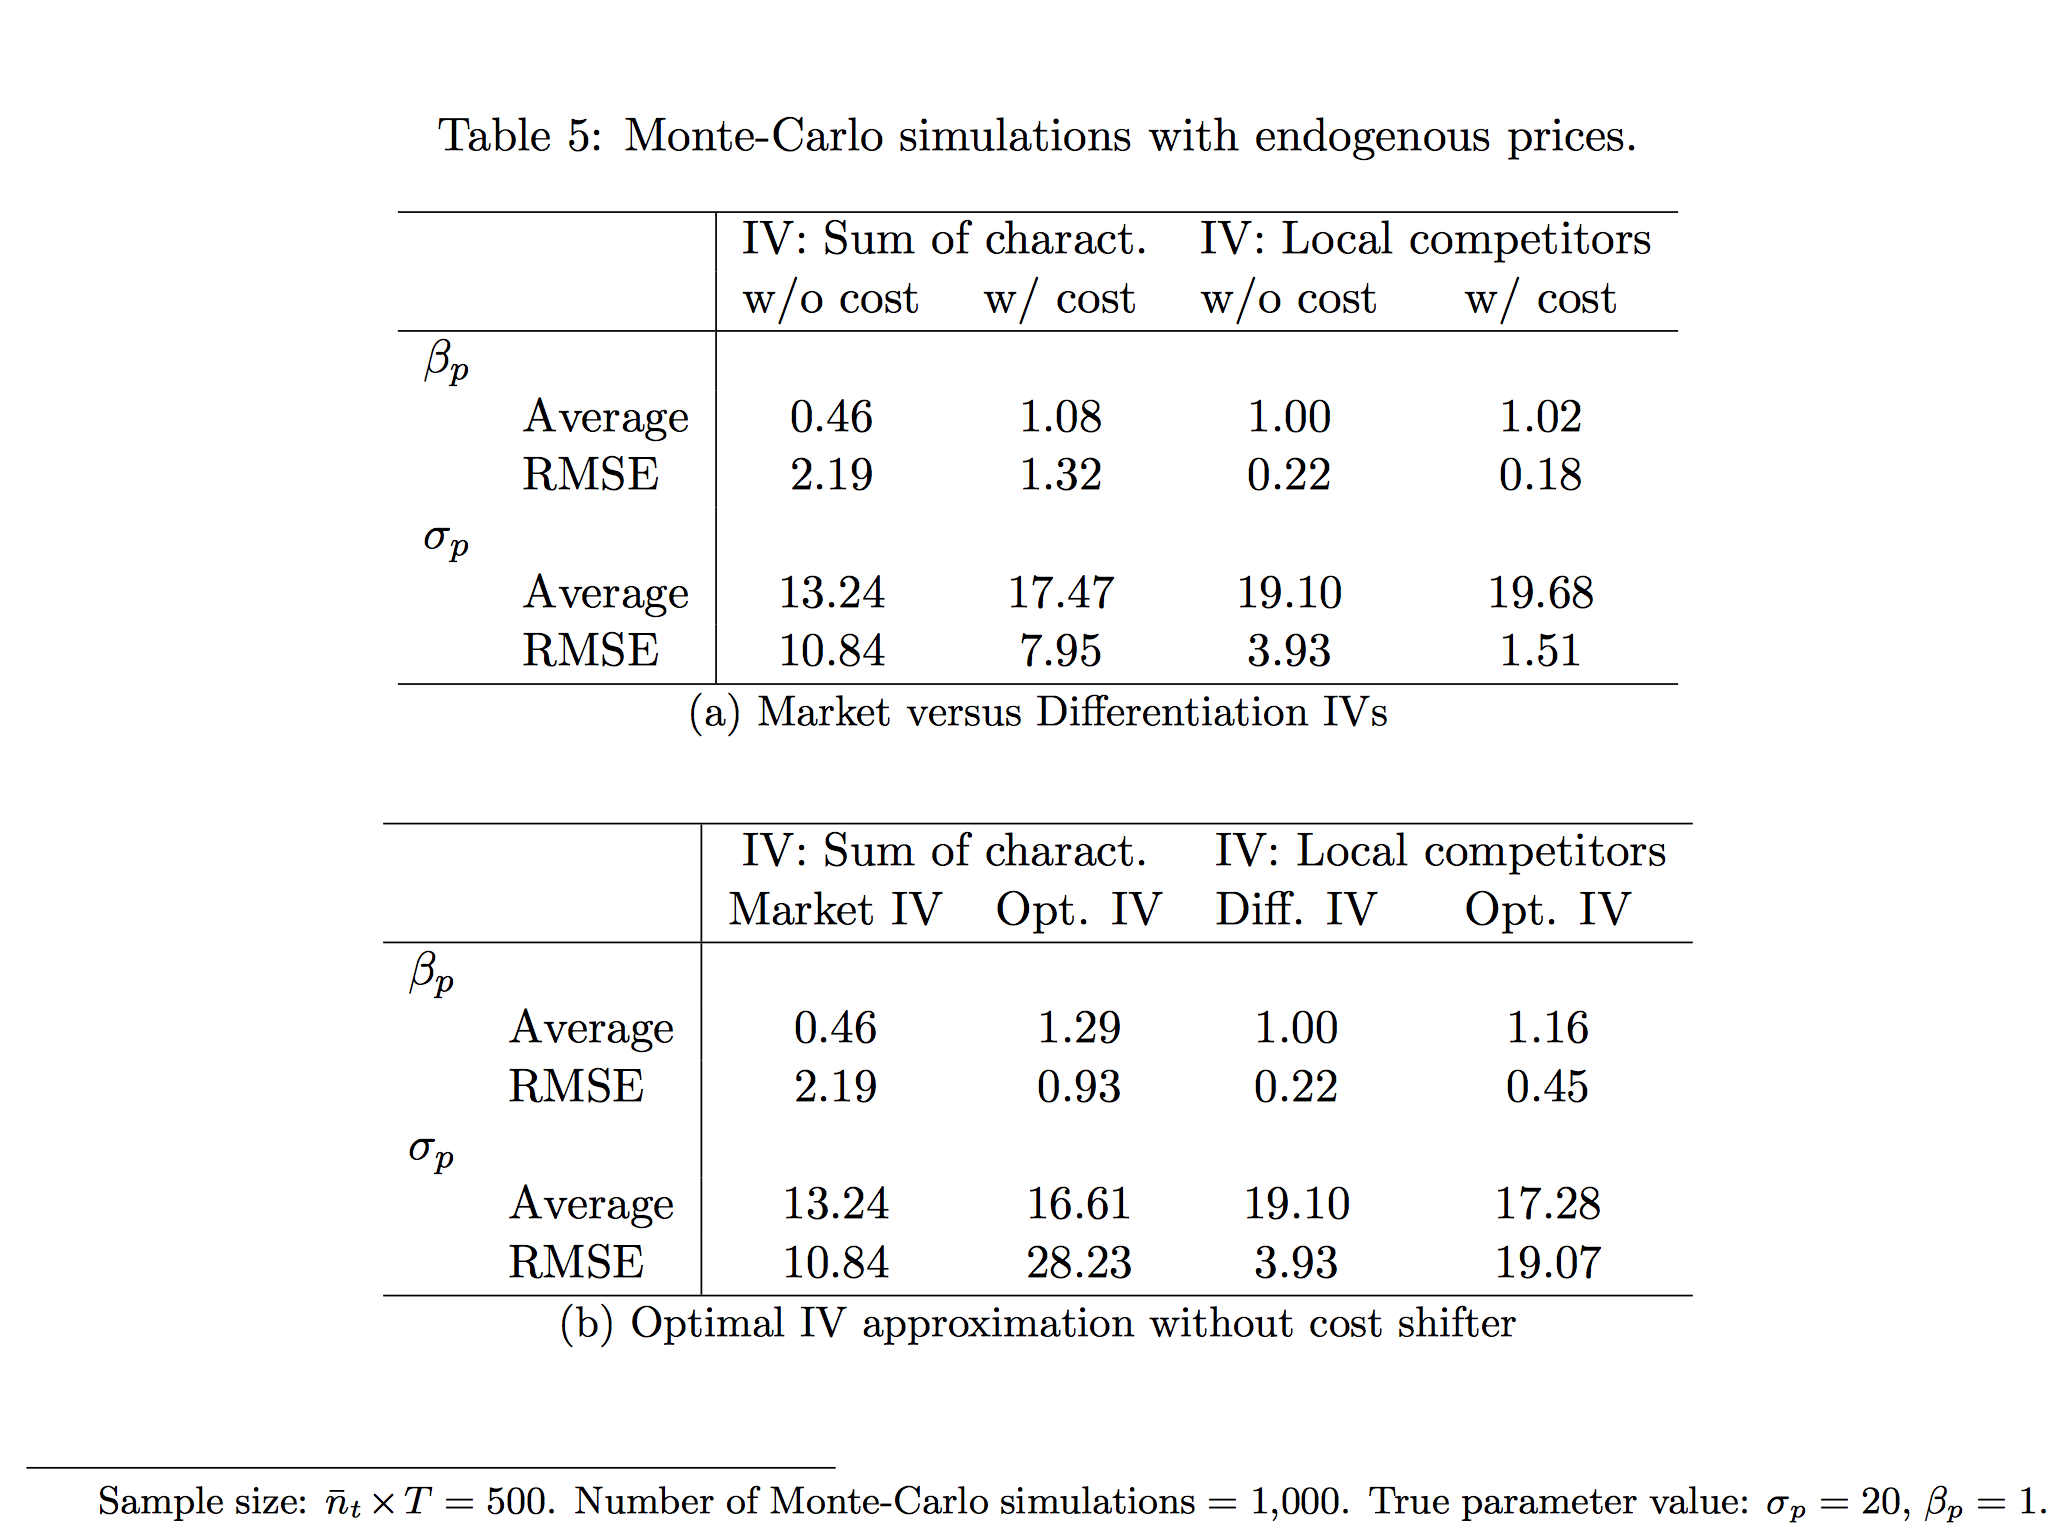
\includegraphics[width=4in]{resources/d_iv2.png}
\end{center}
\end{frame}





\end{document}